\documentclass[twoside,11pt]{article}

\usepackage{blindtext}

% Any additional packages needed should be included after jmlr2e.
% Note that jmlr2e.sty includes epsfig, amssymb, natbib and graphicx,
% and defines many common macros, such as 'proof' and 'example'.
%
% It also sets the bibliographystyle to plainnat; for more information on
% natbib citation styles, see the natbib documentation, a copy of which
% is archived at http://www.jmlr.org/format/natbib.pdf

% Available options for package jmlr2e are:
%
%   - abbrvbib : use abbrvnat for the bibliography style
%   - nohyperref : do not load the hyperref package
%   - preprint : remove JMLR specific information from the template,
%         useful for example for posting to preprint servers.
%
% Example of using the package with custom options:
%
% \usepackage[abbrvbib, preprint]{jmlr2e}

\usepackage{jmlr2e}
\usepackage{amsmath}
\usepackage{graphicx}

% Definitions of handy macros can go here

\newcommand{\dataset}{{\cal D}}
\newcommand{\fracpartial}[2]{\frac{\partial #1}{\partial  #2}}

% Heading arguments are {volume}{year}{pages}{date submitted}{date published}{paper id}{author-full-names}

\usepackage{lastpage}
\jmlrheading{23}{2023}{1-\pageref{LastPage}}{1/21; Revised 5/22}{9/22}{21-0000}{Vsevolod Ladtchenko}

% Short headings should be running head and authors last names

\ShortHeadings{Label Alignment for Multiclass Domain Adaptation}{Label Alignment for Multiclass Domain Adaptation}
\firstpageno{1}

\begin{document}

\title{Label Alignment for Multiclass Domain Adaptation}

\author{\name Vsevolod Ladtchenko \email vladtche@uwaterloo.ca \\
       \addr Department of Statistics\\
       University of Waterloo\\
       200 University Ave W, Waterloo ON N2L 3G1, Canada}

\editor{}

\maketitle

\begin{abstract}%   <- trailing '%' for backward compatibility of .sty file
Project for CS 680 Winter 2023.
\end{abstract}

\begin{keywords}
  label alignment, domain adaptation
\end{keywords}

\section{Introduction}

Domain adaptation is the problem of training a model on one set of data, called the source data, and then applyng the trained model on a second set of data, called the target data. The reason for doing this is because in a supervised setting, we have labels for the source data, but we do not have labels for the target data. So a model trained using supervision from the source labels should extrapolate that knowledge to the target data, which has a different distribution. For example, letters drawn by one group of people have a different distribution than letters drawn by a different group of people. We have labels only for the first group, and after our model learns from the first group, we would like it to generalize to the second group. There is no general way to describe the transformation between these distributions. Previously used methods attempt to learn representations that are invariant to the transformation between distributions, and this works for specific cases, see Section 1 of \cite{imani2022label}. 

The method we investigate is a novel approach that relies on a property of the dataset itself. A dataset has the \emph{label alignment} property when the label vector is mostly in the span of the top singular vectors of the data matrix. This means that for a dataset with $n$ samples and $d$ features represented by a matrix of shape $(n, d)$, we can take the Singular Value Decomposition (SVD) of the data matrix, project the label vector on the resulting $d$ singular vectors, and find that a small number $k \ll d$ of singular vectors will contain a majority of the norm of the projection. This label alignment property emerges as a result of columns of the data matrix being correlated to the label vector (see Appendix A of \cite{imani2022label}). This property also emerges in hidden representations of neural networks, meaning the label vector is in the span of the top few singular vectors of the SVD of a weight matrix of a hidden layer of a neural network \cite{imani2022representation}. In particular this happens towards the topmost layers, showing that neural networks transform the input data until it is correlated to the label vector. We will now summarize the most important mathematical derivations of \cite{imani2022label} relevant to our discussion.

In a linear regression setting, we can show that the label alignment property implies a certain structure on the weights (later we will reverse this phenomenon by imposing this structure on the weights to force label alignment with the target domain). If we have a data matrix $\mathbf{X}$ which has $n$ data points, $d$ features, and thus shape $(n,d)$, and a label vector $\mathbf{y}$ of length $n$, the usual linear regression problem is to find weights to minimize the square error:

$$
\begin{aligned}
\mathbf{w}^* &= \operatorname*{arg\,min}_{\mathbf{w}} MSE(\mathbf{w}) \\
&= \operatorname*{arg\,min}_{\mathbf{w}} \lVert \mathbf{X} \mathbf{w} - \mathbf{y} \rVert^2 \\
\end{aligned}
$$

First, replace $\mathbf{X}$ by its SVD. Then left-multiply by $\mathbf{U}^T$ which is a unitary matrix (a rotation), meaning it does not change the norm, nor its square, and $\mathbf{U}^T \mathbf{U} = \mathbf{I}$. 

$$
\begin{aligned}
&= \operatorname*{arg\,min}_{\mathbf{w}} \lVert \mathbf{U \Sigma V}^T \mathbf{w} - \mathbf{y} \rVert^2 \\
&= \operatorname*{arg\,min}_{\mathbf{w}} \lVert \mathbf{\Sigma V}^T \mathbf{w} - \mathbf{U}^T \mathbf{y} \rVert^2 \\
\end{aligned}
$$

Since $\mathbf{w}$ is a vector of length $d$, and $\mathbf{V}$ is a basis for $\mathbb{R}^d$, then $\mathbf{V}^T \mathbf{w}$ is a projection of $\mathbf{w}$ on the basis spanned by $\mathbf{V}$. Since $\mathbf{\Sigma}$ is a diagonal matrix, we multiply the $i^{th}$ element of $\mathbf{V}^T \mathbf{w}$, or $\mathbf{v}_i^T \mathbf{w}$, by $\sigma_i$. Similarly, $\mathbf{U}^T \mathbf{y}$ is a projection of $\mathbf{y}$ on the $d$ singular vectors $\mathbf{u}_i$. Altogether, this is vector notation for the following sum:

$$
\begin{aligned}
&= \sum_{i=1}^d (\sigma_i \mathbf{v}_i^T \mathbf{w} - \mathbf{u}_i \mathbf{y})^2
\end{aligned}
$$

It is at this point that we invoke the label alignment property of $\mathbf{y}$. Because $\mathbf{y}$ is spanned mostly by the top $k$ singular vectors $\mathbf{u}_i$, we have $\mathbf{u}_i \mathbf{y} \approx 0$ for $i>k$. This is approximate due to noise. Now we can remove $\mathbf{u}_i \mathbf{y}$ from the above sum for terms $i>k$, yielding: 

$$
\begin{aligned}
&= \sum_{i=1}^k (\sigma_i \mathbf{v}_i^T \mathbf{w} - \mathbf{u}_i \mathbf{y})^2 + \sum_{i=k+1}^d (\sigma_i \mathbf{v}_i^T \mathbf{w} )^2
\end{aligned}
$$

Keep in mind we got this formulation by assuming the linear regression problem, and a dataset that follows the label alignment property. The first term is a linear regression problem in a smaller subspace. The second term is a regularization term on the weights $\mathbf{w}$, because it does not involve the labels $\mathbf{y}$. This is the \emph{label alignment regularization} term, because for a prediction $\mathbf{p} = \mathbf{X w}$, it forces $\mathbf{p}$ to align with the top singular vectors just like $\mathbf{y}$ does:

$$
\begin{aligned}
\mathbf{p} &= \mathbf{X w} &&= \mathbf{U \Sigma V}^T \mathbf{w} \\
\mathbf{U}^T \mathbf{p} &= \mathbf{U}^T \mathbf{U \Sigma V}^T \mathbf{w} &&= \mathbf{\Sigma V}^T \mathbf{w}\\
\mathbf{u}_i^T \mathbf{p} &= \sigma_i \mathbf{v}_i^T \mathbf{w}\\
\end{aligned}
$$

By minimizing the right hand side, we minimize the projection of $\mathbf{p}$ on the singular vectors $\mathbf{u}_i$ for $i>k$, which makes $\mathbf{p}$ lie in the span of the top singular vectors of $\mathbf{X}$. Since this term does not require $\mathbf{y}$, we can create a similar term for the target dataset $\mathbf{\tilde{X}}$, which will make $\mathbf{p}$ lie in the span of the top singular vectors of $\mathbf{\tilde{X}}$. This is the main argument of \cite{imani2022label}, which improves domain adaptation by making a model trained on source data have its output lie in the same span as the unknown target label $\mathbf{\tilde{y}}$.

Denote the SVD of $\mathbf{\tilde{X}}$ as $(\mathbf{\tilde{U}}, \mathbf{\tilde{\Sigma}}, \mathbf{\tilde{V}}^T)$, then the regularizer is $\sum_{i=k+1}^d (\tilde{\sigma}_i \mathbf{\tilde{v}}_i^T \mathbf{w} )^2$. It imposes structure on $\mathbf{w}$, which, based on the previous derivation, again implies the linear regression problem and the label alignment property of the target dataset, except we do not need to know the label this time. \cite{imani2022label} has shown promise empirically in using this method to transfer knowledge from the source domain to the target domain. It only assumes the target domain has the label alignment property (which is fair if it is similar to the source domain), and a specific $k_t$ which may differ from $k_s$ of the source domain. For some derivations of $k$ on real world datasets, see Table 1 in \cite{imani2022label}. 

\section{Extensions}

\subsection{Linear Multiclass}

For classification, \cite{imani2022label} applies the regularization technique to classifiers with just two classes. The pressing question is whether the technique extends to multiple classes. To answer this, we investigate in detail the problem of domain adaptation applied to MNIST being the source data, and USPS being the target data, which both have 10 classes. 

The first order of business is to figure out if this dataset has the label alignment property. Since the label $\mathbf{y}$ is a vector of integers corresponding to the handwritten numbers, such a format implies a regression problem. We convert it to a one-hot encoded matrix $\mathbf{Y}$, with labels $\pm 1$. This choice yields higher label alignment $\mathbf{U}^T \mathbf{y}_i$ than using $\{0,1\}$, according to \cite{imani2022label}. Then we project each column of the one-hot matrix onto the basis $\mathbf{U}$ and find that it does indeed have large components in the top singular vectors, as seen in \ref{fig:cumulative_norm}. This makes sense because each one-hot vector can be seen as a binary one-vs-many classification, and \cite{imani2022label} has shown that creating a binary classifier from any two numbers, which would be a subset of this vector, already works. 

\begin{figure}[htbp]
  \centering
  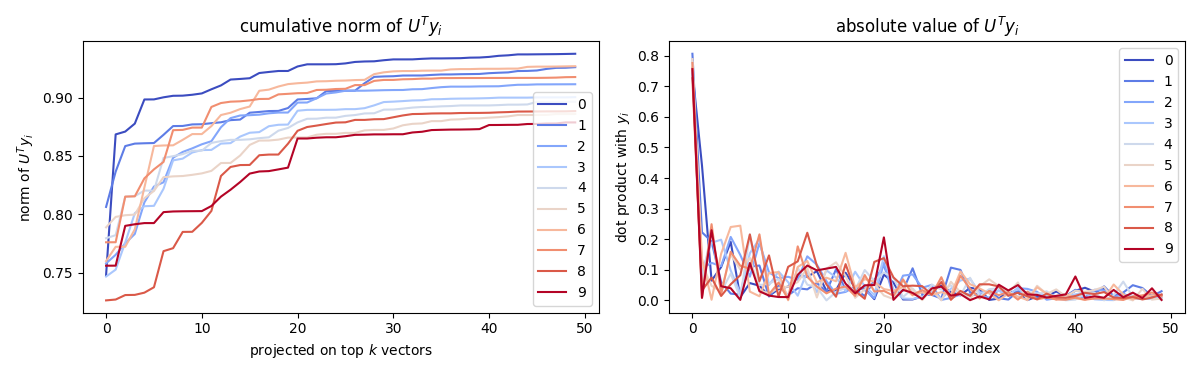
\includegraphics[width=1.0\textwidth]{img/cumulative_norm.png}
  \caption{Cumulative norm of the one-hot labels $\mathbf{y}_i$ projected onto $\mathbf{U}$. The left plot demonstrates that over 70\% of each label's norm is spanned by just the first singular vector. The right plot shows their components, which start very high, have some decently high values in the first 20 singular vectors, and then taper down to noise.}
  \label{fig:cumulative_norm}
\end{figure}

We start by training a basic linear model, which is a $(785, 10)$ matrix multiplication $\mathbf{W}$. Without regularization, it achieves 86\% accuracy on the source test set, and 10\% on the target test set, which is as good as a random guess. When we add the regularization, with naive parameter choices $k=3, \lambda=10^4$, we get a target test accuracy of 35\%.

\subsection{Choice of $k_s, k_t, \lambda$}

The regularization weight $\lambda$ has to be found using a grid search for every new model and combination of $k_s, k_t$. 

In regards to $k$, we see in \ref{fig:cumulative_norm} that each one-hot label vector is mostly in the span of a different number of top singular vectors. For example, in the left figure, if we look at the horizontal line at 0.85 norm, we see that a label vector can have 85\% of its norm be spanned by between 2-20 singular vectors. This suggests using a different $k_i$ for each one-hot label vector. \cite{imani2022label} suggests choosing the smallest $k$ such that the norm of the first $k$ components will be 90\% of the total projected norm. We implemented this by choosing such a $k_i$ for each one-hot label vector, and creating a mask. Multiplying the mask by $\mathbf{\Sigma V}^T \mathbf{W}$ will zero out the elements $1$ through $k_i$ of column $i$, and as a result the regularization term will take a different sum (from $k_i + 1$ to $d$) for each column. As a result, our accuracy went down to 30\%, suggesting we cut out important vectors, and that important vectors may have small components. We thus abandon the $k_i$ and return to the idea of a single $k$ for each distribution.

For the problem of hard thresholding of singular values, \cite{brunton_kutz_2019} suggest a technique developed by \cite{gavish2014optimal} which is based on estimating the SVD of a pure noise distribution, with singular values $\mathbf{\Sigma}_{noise}$, and choosing the first $k$ singular values from our target distribution which will be $\geq \max(\mathbf{\Sigma}_{noise})$. We apply this technique to the target distribution to yield $k_t = 96$. We did not apply this technique to the source distribution, as discussed below.

It is at this point that we would like to discuss the difference in interpretation between the regularizer applied to the source and the target, as described by \cite{imani2022label}. As discussed previously, the interpretation of the regularizer is that minimizing the right hand side makes our prediction roughly orthogonal to all but the top few singular vectors.

$$
\begin{aligned}
\mathbf{u}_i^T \mathbf{p} &= \sigma_i \mathbf{v}_i^T \mathbf{w}\\
-\sum_{i=k+1}^d (\sigma_i \mathbf{v}_i^T \mathbf{w} )^2 &= -\sum_{i=k+1}^d (\mathbf{u}_i^T \mathbf{p} )^2\\
\end{aligned}
$$

This holds for the target distribution regularizer, which is a positive term. But \cite{imani2022label} also subtract this regularizer as applied to the source data. The reason for subtracting it is to remove its implicit existence inside the MSE objective. But we arrived at this term with the approximate assumption that $\mathbf{u}_i^T \mathbf{y} \approx 0$. Therefore it is unclear whether this has the desired consequence of removing the implicit term. What it does introduce, however, is a different interpretation. An algorithm minimizing this term would seek to maximize the absolute dot product $\mathbf{v}_i^T \mathbf{w}$. This makes the relationship between $\mathbf{p}$ and $\mathbf{u}_i$ unclear, as now they will be parallel to each other. 

First, we would like to see if the source regularizer has a negative impact on the optimization. We perform a side experiment with a synthetic dataset recreated from the description in \cite{imani2022label}, a simple 2-dimensional classification. The classifier finds the target saparating hyperplane with $\lambda = 10$. Removing the source regularizer does not change the loss graph nor hyperplane, suggesting the source regularizer is not essential.

Next, we return to the handwritten digits problem to investigate the effect of the source regularizer. We note that here the source regularizer is parametrized by $k_s$, so to investigate the relationship between $k_s, k_t$ given $\lambda$, we try 6 experiments \ref{fig:ks_vs_kt}. Each experiment has a set value of $\lambda$, and we iterate over 10 possilble values of both $k_s$ and $k_t$. To create the plots, we condition the resulting data on $k_s$, leaving us with a plot of $k_t$ against accuracy, given a set value of $k_s$ and $\lambda$. 

Trying different values of $k_s, k_t$ shows that they have a volatile relationship, which may have to do with the similarity of the singular vectors between the two distributions. This is especially true for lower values of $\lambda$ where the target regularizer does not overpower the source. In this case, the source regularizer has a large impact since it is not bounded below, like the target regularizer is. This raises the question of whether our prediction $\mathbf{p}$ is becoming orthogonal to the target singular vectors via the minimization of $(\tilde{\sigma}_i \mathbf{\tilde{v}}_i^T \mathbf{w})^2$, or aligning with the source singular vectors via the minimization of $-(\sigma_i \mathbf{v}_i^T \mathbf{w})^2$.

For high values of $\lambda$, the influence of $k_s$ mostly disappears, which makes sense as it is the relative weight. For lower values of $\lambda$ its effect is nonlinear and dependent on $k_t$. This clarifies that $k_s, k_t$ have a relationship that is not easy to interpret. It adds volatility for low values of $\lambda$, and is overpowered for high values of $\lambda$, thus we choose to drop this term. 

Removing the source regularizer makes the resulting parameter landscape with just $k_t, \lambda$ smooth and unimodal. Interestingly, lower values of $\lambda$ favor lower values of $k_t$, while higher values of $\lambda$ favor higher values of $k_t$. At $\lambda = 10^9$ we see hints of numerical instability, where the loss is jumping around too much. 

\begin{figure}[htbp]
  \centering
  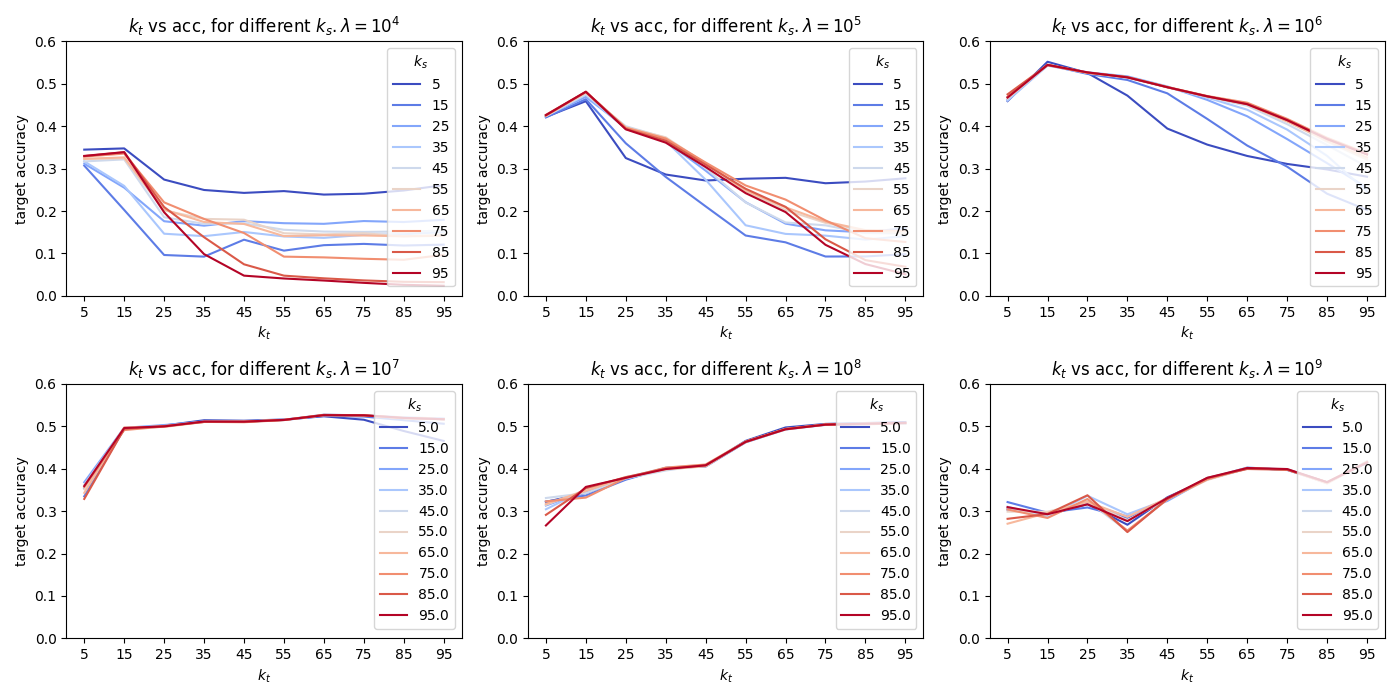
\includegraphics[width=1.0\textwidth]{img/k1_vs_k2.png}
  \caption{plot of $k_t$ vs accuracy for different values of $k_s, \lambda$}
  \label{fig:ks_vs_kt}
\end{figure}

Combining the result of \cite{gavish2014optimal}, which gives $k_t = 96$, and removing the source regularizer, thus eliminating the need for $k_s$, yielded an accuracy of a whopping 52\% at $\lambda = 10^7$. Previously, a grid search yielded an absolute maximum of 57\% with $(k_s = 0, k_t = 13, \lambda=10^6)$. Based on the above discussion, this seems like a lucky mistake, as it is hard to interpret the source regularizer, as well as why $k_s = 0$ works well.  

\section{Generalization}

The derivation of the regularizer only depends upon the assumption that $\mathbf{u}_i^T \mathbf{y} \approx 0$ for $i>k$, which is a property of the dataset. Let us consider a general function $\mathbf{f}(\mathbf{w})$, which is a vector of size $n$. We can once again left-multiply by $\mathbf{U}^T$, and invoke the label alignment property:

$$
\begin{aligned}
\lVert \mathbf{f} (\mathbf{w}) - \mathbf{y} \rVert^2 &= \lVert \mathbf{U}^T\mathbf{f} (\mathbf{w}) - \mathbf{U}^T\mathbf{y} \rVert^2 \\
&= \sum_{i=1}^d \bigl( \mathbf{u}_i^T \mathbf{f} (\mathbf{w}) - \mathbf{u}_i^T \mathbf{y} \bigr)^2 \\
&= \sum_{i=1}^k \bigl( \mathbf{u}_i^T \mathbf{f} (\mathbf{w}) - \mathbf{u}_i^T \mathbf{y} \bigr)^2 + \sum_{i=k+1}^d \bigl( \mathbf{u}_i^T \mathbf{f} (\mathbf{w}) \bigr)^2 \\
\end{aligned}
$$

We propose the right term on the last line as a generalization of the regularizer by \cite{imani2022label}. As expected, it has identical performance on the linear problem when $\mathbf{f} (\mathbf{w}) = \mathbf{X w}$. It also has the same interpretation, that minimizing the RHS makes our prediction orthogonal to all but the top few singular vectors:

$$
\begin{aligned}
  \mathbf{p} &= \mathbf{f} (\mathbf{w}) \\
  \mathbf{u}_i^T \mathbf{p} &= \mathbf{u}_i^T \mathbf{f} (\mathbf{w}) \\
\end{aligned}
$$

\subsection{Tanh Regression}

A first experiment is to try a simple logistic regression, with the activation function replaced with \texttt{tanh} since we use $\pm 1$ encoding. Without any regularization, this model achieves 40\% on the target test set. When applying generalized regularization, we do not include a source regularization term (when we try it later, it hinders performance, and creates volatility). A grid search yields 53\% accuracy with $k_t = 13, \lambda=10^5$, suggesting that this is the highest we can achieve with linear decision boundary models. 

Logistic (and similarly \texttt{tanh}) regression work as squashing functions, taking the output of a matrix multiplication and bringing it closer to our labels $\{\pm 1\}$. They do not otherwise transform the data. Under this interpretation, linear and logistic models are very functionally similar. This suggests trying the original \emph{linear} regularizer for our \texttt{tanh} regression. This experiment yielded 40\% which did not beat \texttt{tanh} without regularization.

Next we try a neural network with one hidden layer of 400 units. It achieves 57\% test accuracy without regularization. But upon applying the generalized regularization, its test performance drops to 10\% for most hyper parameter values. This is interesting, considering this regularizer can make a linear regression go from 10\% to over 50\%, but makes a neural network go from over 50\% to 10\% by just adding one hidden layer. This is a topic that deserves further investigation.  

\section{Discussion}

In this project our main objective is to extend the results of \cite{imani2022label} for the multiclass case. We work with the handwritten digits dataset, specifically with MNIST as the source data, and attempt to transfer the learned model to the USPS data. To get a feel for the task, we plot some sample data points in \ref{fig:data_sample}. 

Handwriting style aside, the target distribution has different qualitative features. We had to scale up the images from the USPS dataset to match the dimensions of the MNIST data, which introduces additional antialiasing pixels. Additionally, the USPS digits are stretched to the borders, while MNIST has a border of empty pixels. This loses some information, as one can imagine a convolutional network would not be seeing all the relevant edges of a number. A linear model would struggle more, as it inherently assumes the same interpretation for each pixel. For example, a linear regression model on health data would treat each input $x_i$ as a separate risk factor. But in our problem, no pixel $x_i$ has a standardized interpretation because letters are subject to transformations such as rotation, scale, and translation \cite{brunton_kutz_2019}. Because linear models cannot easily understand such transformations, achieving any degree of success with them is remarkable. In particular, the source data will not teach them about border pixels, since they are mostly empty, only the regularization term \emph{might}.

\begin{figure}[htbp]
  \centering
  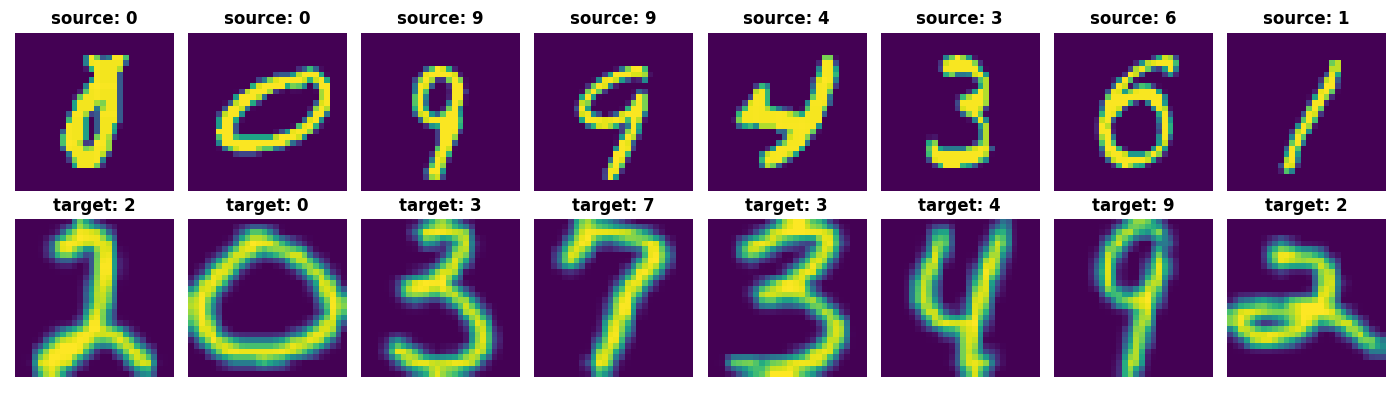
\includegraphics[width=1.0\textwidth]{img/data_sample.png}
  \caption{Sample points from the source and target datasets.}
  \label{fig:data_sample}
\end{figure}

In choosing parameters $(k_s, k_t, \lambda)$ we discuss the questionable efficacy of the source regularizer. It adds volatility to the loss surface, and therefore the few times that it appears helpful are viewed with suspicion. Removing it makes the loss surface unimodal, and easier to interpret by doing a grid search over $(k_t, \lambda)$. The technique suggested by \cite{gavish2014optimal} gives us a value $k_t = 96$. One might question whether this value is too large, but the fact that it can achieve maximum possible accuracy together with a certain $\lambda$ shows us that it is not just random noise. 

While working with the regularizer, we tried non-linear models. Trying to theoretically justify its use proved fruitless, but instead allowed us to realize that the model is unrelated to its derivation. Thus we introduced a generalization of the regularizer for non-linear models. It shows success with logistic regression, achieving the same maximum accuracy as the linear model. This brings up the question of whether there is a cap to how much knowledge we can transfer over from the source domain. 

Such a cap is definitely model dependent, as one can imagine a convolutional network doing very well. For linear models, we have not found a way to surpass the fifty percent range. Going over to neural networks, the generalized regularizer (and its variants) not only hurt performance but brought it all the way from 57\% to \emph{random guess} level of 10\%. This is remarkable in its own way because there is definitely something going on. It seems that the addition of a hidden layer has caused the singular vectors $\mathbf{u}_i$ to lead the solution astray, and the reason why is worth looking into.

\section{Future Work}

Due to time and GPU cooling constraints, we were not able to run all of the planned experiments involving more varieties of models and hyperparameters. Aside from that, there is also more work to be done in investigating the efficacy of the regularization term for non-linear models. Despite our lack of success with neural networks, \cite{imani2022representation} describe how the label vector lies in the span of the top few singular vectors of the hidden representation matrix of neural networks. If this regularizer works for the linear case, and the non-linear case shows the same properties, then a relationship must exist. 

Additionally, we focused on one problem of handwritten digits in order to develop techniques and intuition. Using these techniques on other datasets is the next logical step. 

There are broader questions as well. For different \emph{tuples} of datasets, meaning source and target, different relationships may exist between their singular value decompositions. These relationships can be in the form of comparing the amount of high singular values, the dropoff of singular values, and the angles between the most important singular vectors, to name a few. These relationships can have direct influence on the success of domain adaptation. Due to the generality of these statements, it is important to set up a baseline of synthetic datasets from which to draw intuition. Afterwards, we can take real world datasets, see the relationsip between their SVDs, and map this relationship to a synthetic experiment that we analyzed earlier, to draw inferences. 

% Manual newpage inserted to improve layout of sample file - not
% needed in general before appendices/bibliography.

\appendix

% \section{}

% \label{app:theorem}

% Note: in this sample, the section number is hard-coded in. Following
% proper LaTeX conventions, it should properly be coded as a reference:

%In this appendix we prove the following theorem from
%Section~\ref{sec:textree-generalization}:

% \noindent

% \noindent

% \vskip 0.2in

\bibliography{sample}

\end{document}
